\documentclass{article}
\usepackage[utf8]{inputenc}
\usepackage{amsmath}
\usepackage{amsfonts}
\usepackage{enumitem}
\usepackage{amssymb} 
\usepackage{xcolor}
\usepackage{soul}
\usepackage{todonotes}
\usepackage[margin=2.5cm]{geometry}
\graphicspath{ {./images/} }

\title{Heaps}
\author{Jin Long Cao, Ethelia Choi}
\date{October 2022}

\begin{document}
\maketitle
\section*{Implementing a Combined MinHeap and MaxHeap Data Structure}
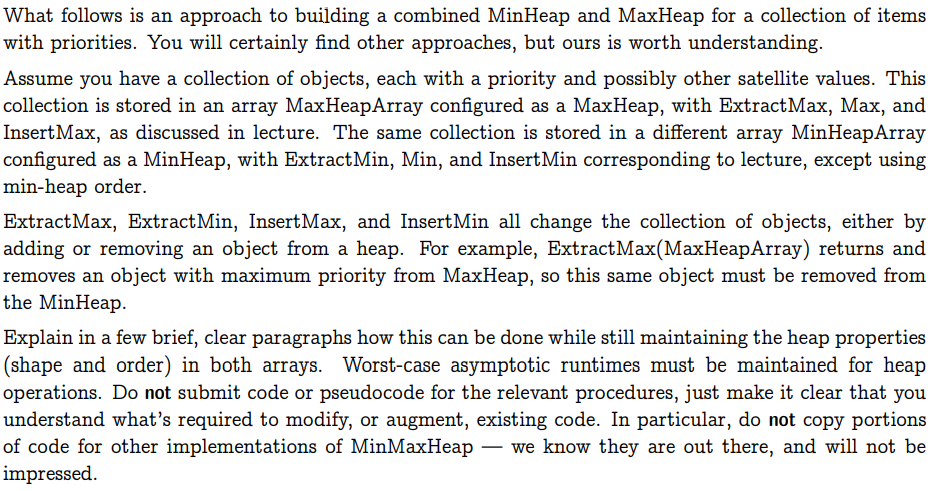
\includegraphics[width=\textwidth]{Heaps2}
\section*{Solutions}
% The goal is to build a combined MinHeap and MaxHeap for a collection of items with priorities. 
When we consider the process of extracting the max element from a MinHeapArray, recall that in a MinHeapArray, the two pieces of information we know are that a) the min element is at the root, and b) every parent has a value smaller than its children. In other words, we do not know where the max element is. Our best bet would be to loop over every element in the array and compare, which will obviously take a long time. \\~\\
Suppose we found the max element in the MinHeapArray, we need to swap it with the last element in the array, decrement the heapsize by 1 and bubble up until Min-heap-order is restored. This will take $O(\lg n)$. However, the entire function ExtractMax should only take $O(\lg n)$. Thus, in order to preserve the time complexity, we will need a way to quickly find the max element, in $O(1)$. To do this, our approach is to alter the way we insert an element into a MinHeapArray. (The same issue will arise when we want to extract the min element from a MaxHeapArray. So we will also need to change the way we insert into a MaxHeapArray). 


\subsubsection*{InsertMax, InsertMin}
% Insert the desired element at index heap-size + 1, increase the heap-size by 1, and swap with parent until max-heap order restored (bubble up). Which is the way it has been explained in class and has a worst-case runtime of $O(\lg n)$. 

When we insert an element into a MaxHeapArray, we will make the element have a satellite value that stores a pointer. This pointer will tell us where this element is in the MinHeapArray, since we will insert it into the MinHeapArray as well. The operation of InsertMax basically works the same as explained in class: we will add the element (with its priority and pointer value) at index heap-size + 1, increment heap-size by 1, and then swap with parents until the max-heap order is restored (heapify). The only difference is that the element holds more information now. Adding the pointer will take $O(1)$. Since we can access the heap-size through the satellite value Q.heap-size, adding the element and incrementing heap size will take $O(1)$. At last, heapify takes $O(\lg n)$. Altogether, InsertMax has a worst-case runtime of $O(\lg n)$. \\~\\
We also insert the same element into the MinHeapArray. This element will have a satellite value that stores the pointer that points to its location in the MaxHeapArray. The rest of inserting works like the opposite of InsertMax: We add the element (with it's priority and pointer value) at index heapsize + 1, increment heapsize by 1, and then swap with parents until min-heap order restored (heapify). Since it's similar to inserting in Max-heap, the worst-case runtime is $O(\lg n)$. \\~\\
Now notice that for an arbitrary element in the MaxHeapArray, we can access its location in the MinHeapArray in $O(1)$. Same for an arbitrary element in the MinHeapArray. If we picture this, we have a Max heap and a Min heap side-by-side, then suppose we have an element $a$. Then we will have two $a$'s, one in each heap, and they will point at each other. 

% Similarly, if we want to ExtractMin(MinHeapArray), we return and removes an object with minimum priority from MinHeap. Which has a worst-case runtime of $O(\lg n)$. We would also extract the same element in the Max-Heap. Using the pointer of the element...

\subsubsection*{ExtractMax}
\underline{on MaxHeapArray}\\
\noindent
When we want to ExtractMax on a MaxHeapArray, we return and remove an object with maximum priority from MaxHeapArray. This is done by swapping the first element, Q[1], in the array with the last element of the array, Q[heap-size], decreasing heap-size by 1, and bubble down (heapify). Which is the same way it has been explain in class and has a worst-case runtime of $O(\lg n)$. 

\bigskip\noindent
\underline{on MinHeapArray}\\
We would also want to extract the same element in the MinHeapArray. Since we have a pointer to the element, finding the same element in Min-Heap will cost $O(1)$. Once the element is found, we swap it with the last element of the array, decrease heap size, and heapify. Note that since we have a new satellite value, the pointer, when we relocate the last element, we will need to update the pointer of the same element in the MaxHeapArray. \\~\\
Swapping elements will take $O(1)$ since it is just indexing. Decreasing heap-size will also take $O(1)$ because we can access heap-size through the satellite value, Q.heap-size. Heapify will take $O(\lg n)$. Updating the pointer takes $O(1)$ because we will know its index after heapifying and accessing the pointer will take constant time. Altogether, running ExtractMax on a MinHeapArray will have a worst-case runtime of $O(\lg n)$. 

\subsubsection*{ExtractMin}
\underline{on MinHeapArray}\\
\noindent
We will assume it works the same as ExtractMax on a MaxHeapArray except that we have $\leq $ instead of $\geq$ in the relationship between a parent and its children. Since the operation is basically the same, we can also assume it has the same worst-case runtime as ExtractMax on a MaxHeapArray, which is $O(\lg n)$.

% \bigskip\noindent
% The worst-case runtime will be $O(\lg n)$. This is because it takes 1 step to remove the minimal element, which is at the root. Then, when we bubble up, at most we will have to do this for every level of the tree. So this will take O of the height of the tree, which is $\lg n$.

\bigskip\noindent
\underline{on MaxHeapArray}\\
Now we want to extract the min element from a MaxHeapArray. Since when we insert an element, we created pointers, we can use them to find out exactly where the min element is in the MaxHeapArray. So finding the element only takes $O(1)$. Then, we will swap it with the last element of the array, decrease heap-size by 1, and bubble down accordingly (heapify). Similarly, after we relocate the last element, we will need to update the value of the same element in the MinHeapArray. \\~\\
This operation is the opposite of what we did in ExtractMax on a MinHeapArray. Thus, the runtime will be the same. Altogether, ExtractMin on a MaxHeapArray will have a worse-case runtime of $O(\lg n)$.  
\newpage
\section*{MaxHeap Implementation Issue}
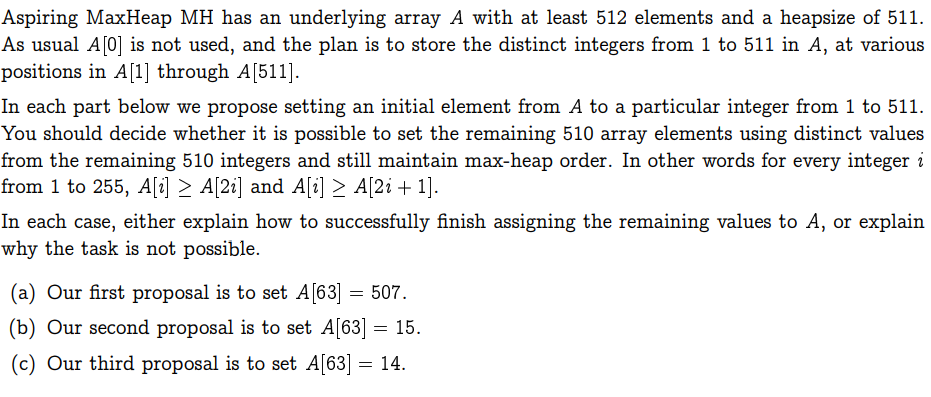
\includegraphics[width=\textwidth]{Heaps1}
\section*{Solutions}
To decide whether it is possible to set the  remaining 510 array elements and still maintain max-heap order. We have to figure out if there are enough ancestors and descendants such that the max-heap order holds. 
% [1, 2, 3, 4, 5, 6, 7, 8, 9, 10] 
% heap size 10

%       10
%    9          8
% 7 6          5  4
% 1 2 3

%       10
%    9          3
% 8 7          2  1
% 6 5 4
% Q([10,9,3,8,7,2,1,6,5,4,?,?,?], 10)
\subsection*{(a)}
Our first proposal is to set $A[63] = 507$.\\
We need to figure out if there are enough elements with higher priority to fill up all the ancestors. \\
Always want the parent to have a greater value than the children. \\
We know A[1] = 511 and $A[1] \geq A[3] \geq A[7] \geq A[15] \geq A[31] \geq A[63] = 507$.\\
We need 5 elements with greater priority than 507 to fill up the 5 ancestor positions, but we know there only exist 4 numbers bigger than 507, namely, 511, 510, 509, and 508. \\
Hence it is not possible to set the remaining 510 array elements using distinct values
from the remaining 510 integers and still maintain max-heap order.

\subsection*{(b)}
Our second proposal is to set $A[63] = 15$.\\
We already know A[1] = 511 and $A[1] \geq A[3] \geq A[7] \geq A[15] \geq A[31] \geq A[63] = 15$.\\
Clearly, there are enough elements with higher priority to fill up all the ancestors. \\
Now we need to figure out if there are enough elements with lower priority to fill up all the descendants.\\
The descendants of $A[63] = 15$ are \\
$A[126], A[127], A[252], A[253], A[254], A[255], A[504], A[505], A[506], A[507], A[508], A[509], A[510], \text{ and } A[511]$\\
Hence, we need 14 elements with a lower priority than $A[63]$, which is 15. Since we have exactly 14 elements with such property, it is possible to set the remaining 510 array elements and still maintain the max-heap order.

   %               63
   %         126         127
   %      252  253     254  255
   % 504 505 506 507 508 509 510 511

\subsection*{(c)}
Our third proposal is to set $A[63] = 14$.\\
Since we know there are 14 descendant positions and only 13 elements with a lower priority to $A[63]$. It is not possible to set the remaining 510 array elements and still maintain max-heap order.
% 1+2+4+...+256=511 (Therefore complete binary tree)

\end{document}